\section{Optimizing Object Tracking}
\label{sec:methods/section_b}

Object tracking pipeline consists of YOLOv3 and SORT, and using the softwares from \cite{jocher_ultralyticsyolov3_2021} and \cite{abewley_abewleysort_2021}, there are 6 parameters needed to be set to run the object tracking. In order to run these softwares, we have to set the suitable parameters, hence, I set the appropriate parameters by optimizing the detection performance for YOLOv3 and tracking performance for SORT. The following parameters needed to be set for YOLOv3 are as follows.
\begin{itemize}
    \item \textbf{Image size}: This parameter is the image resolution for inference of object detection in the YOLOv3 model.
    \item \textbf{Confidence threshold}: This parameter indicates the threshold of object detection. The higher the threshold, the object detector will less likely to detect the target but also less mistakes in detection.
    \item \textbf{IOU threshold for Non-maximum suppression (NMS)}: NMS prevents multiple detections on the same target \cite{redmon_you_2016}. IOU threshold is used in applying NMS in our YOLOv3.
\end{itemize}
For the image size parameter, any input image will be resized to this resolution for prediction. Since the resolution of 640x640 was used in training the pre-trained network weight, we speculated that the detection performance will be the most optimized in that resolution during the inference in testing samples; therefore, we chose 640x640 as an image size.

For the confidence threshold and IOU threshold for NMS, I apply the grid search method to determine the suitable values. To tune these parameters, I run YOLOv3 and SORT on the selected training sequence of Class C PartyScene. Since both parameters range from 0 to 1, I run the detector with a step size of 0.05, and plot the detection performance $F1$ over different confidence threshold and IOU threshold as shown in Figure \ref{fig:F1_vs_conf}.
% \begin{figure}[htb]
%   \centering
%   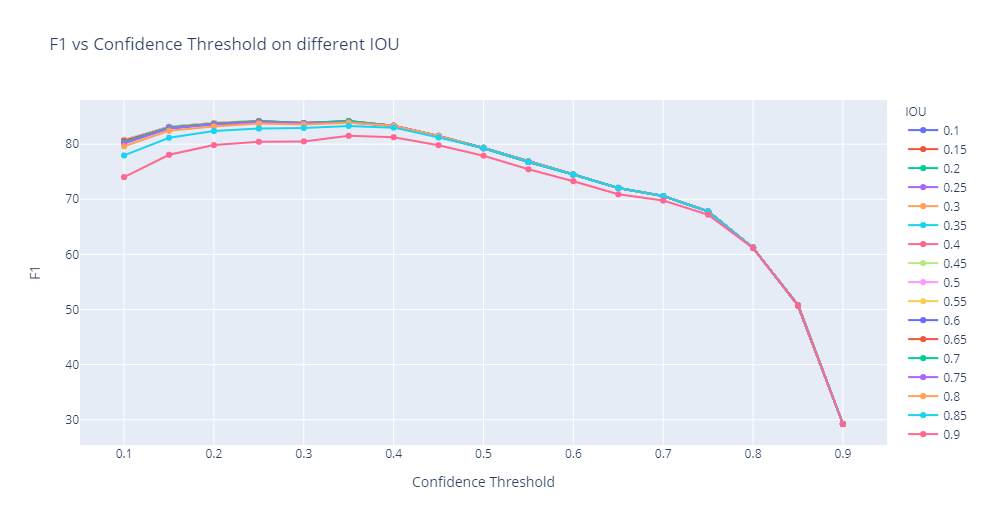
\includegraphics[width=1.0\linewidth]{img/F1_vs_conf_plot.png}
%   \caption[Detection performance F1 over different confidence threshold and IOU threshold for NMS]{
    
%   }
%   \label{fig:F1_vs_conf}
% \end{figure}

\begin{figure}[htbp]
  \centering
  \begin{subfigure}{0.5\textwidth}
    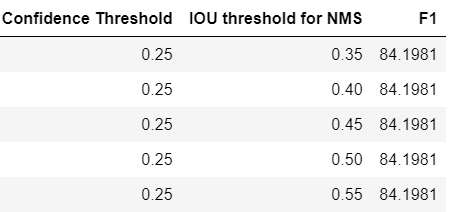
\includegraphics[width=\linewidth]{img/F1_vs_conf_table.png}
    \caption{Highest F1 score on different confidence and IOU threshold}
    \label{fig:F1_vs_conf_table}
  \end{subfigure}
   \begin{subfigure}{1.0\textwidth}
    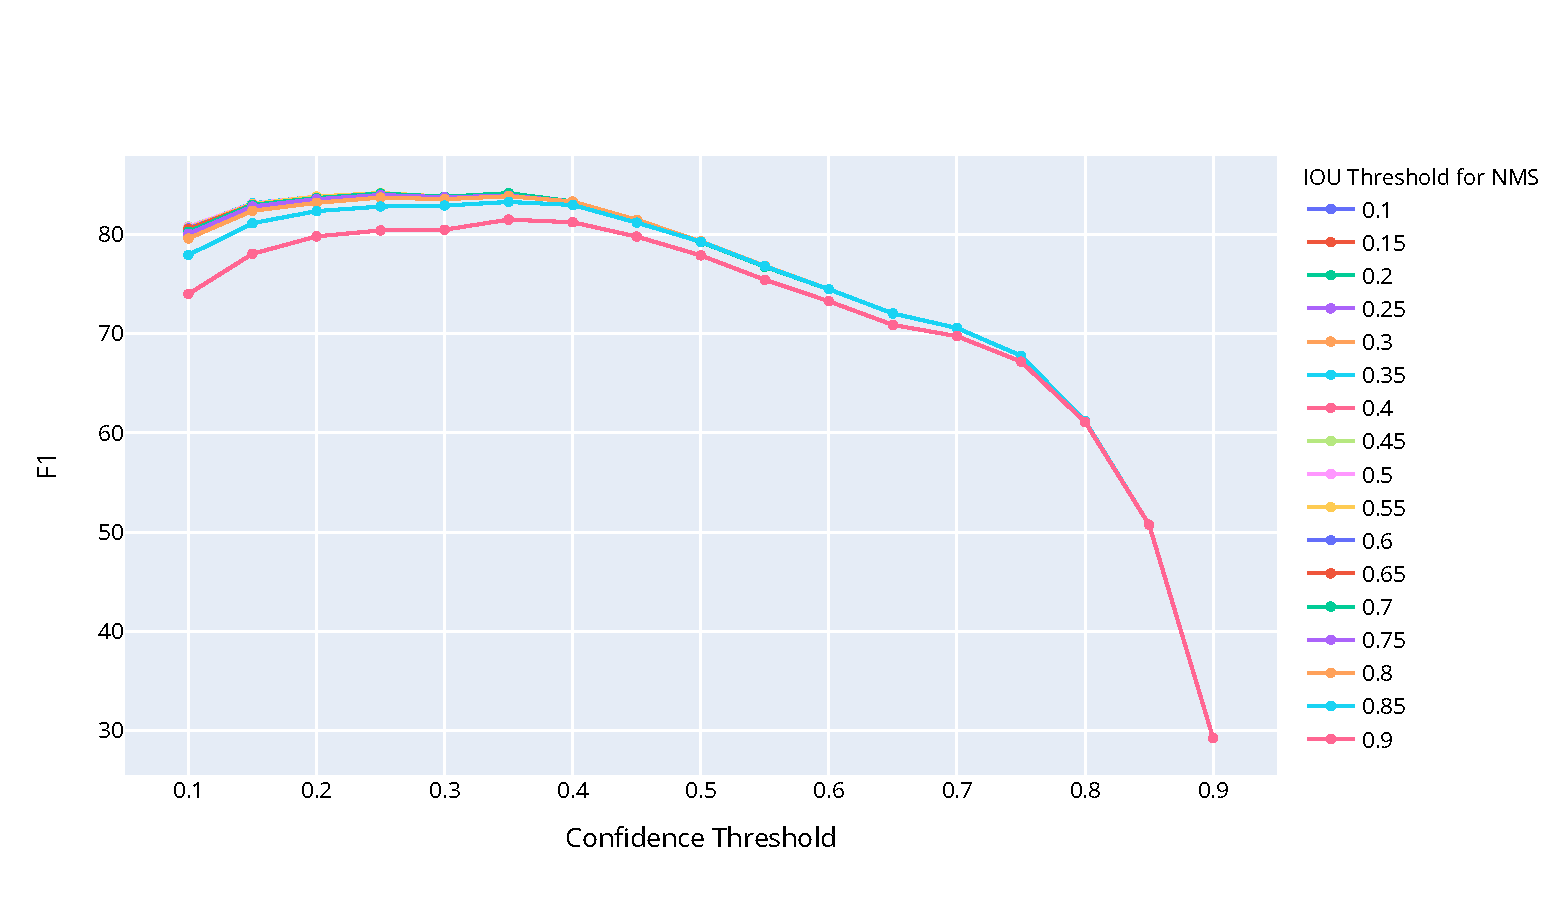
\includegraphics[width=\linewidth]{img/F1_vs_conf_plot.pdf}
    \caption{F1 vs confidence threshold over different IOU threshold plot}
    \label{fig:F1_vs_conf_plot}
  \end{subfigure}
  \caption{}
  \label{fig:F1_vs_conf} % label should be placed below caption
\end{figure}
The table and plot in this figure shows that there are optimal F1 score over different confidence and IOU threshold. The table in (a) shows that the detector achieved the same F1 score over different IOU threshold at confidence threshold of 0.25. Since the higher the IOU threshold we choose, it makes the detector more careful in detection, or in other words, we expect to see less FP and more FN. Therefore, we chose the confidence threshold of 0.25 and IOU threshold for NMS to be 0.55. Note that I also attempted on tuning the parameters based on optimizing mAP but this metric didn't give me insight in finding optimal values of parameters, as explained in Appendix.

For optimizing the tracking performance of SORT, the following input parameters is listed \cite{bewley_simple_2016}.
\begin{itemize}
    \item \textbf{Maximum age}: As T\textsubscript{lost} explained in Chapter \ref{sec:background/section_b}, the value of maximum age determines the maximum number of frames to be alive while no objects are detected before the trajectory termination.
    \item \textbf{Minimum hits}: Minimum number of necessary detections before the trajectory creation and its assignment initialization.
    \item \textbf{Minimum IOU}: Minimum IOU threshold for object matching. IOU less than this threshold indicates that the object doesn't overlap enough with the ground truth, so identity will not be assigned, but assignment takes place when IOU is higher than the threshold.
\end{itemize}
For the maximum age, I chose the value of 1 because \citeauthor{bewley_simple_2016} justified this value by the two reasons; the constant linear motion in Kalman filter framework does not cover the true dynamics where non-linear motion exists and SORT does not deal with the object re-identification \cite{bewley_simple_2016}. For the minimum hits and IOU threshold, I run SORT on the training sequence of Class C PartyScene for both parameters from 0.1 to 0.9 at a step size of 0.05 as a grid search method. Tuning those parameters to optimize the tracking performance, 